\section{Experimental Evaluation}

\subsection{Datasets}


Table~\ref{table:datasets}, shows the summary of the dataset we use for our evaluation. We evaluate on 3 homes, each home having sensors deployed .

\begin{figure}
	\centering
	\begin{subfigure}[b]{0.35\textwidth}
		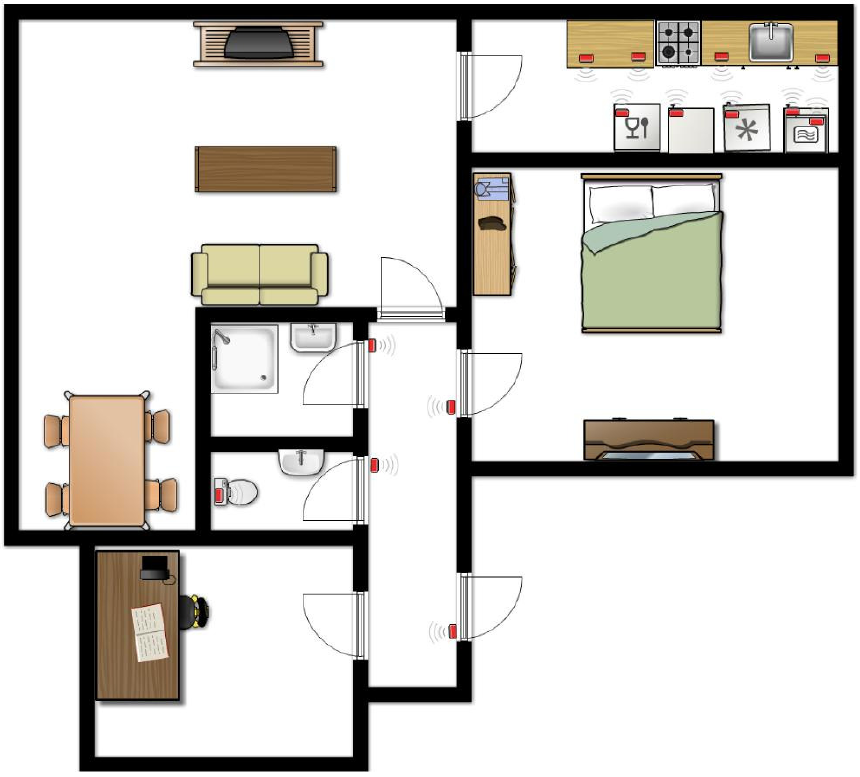
\includegraphics[width=\textwidth]{fig/houseA.png}
		\caption{House A}
		\label{fig:houseA}
	\end{subfigure}
	~
	\begin{subfigure}[b]{0.35\textwidth}
		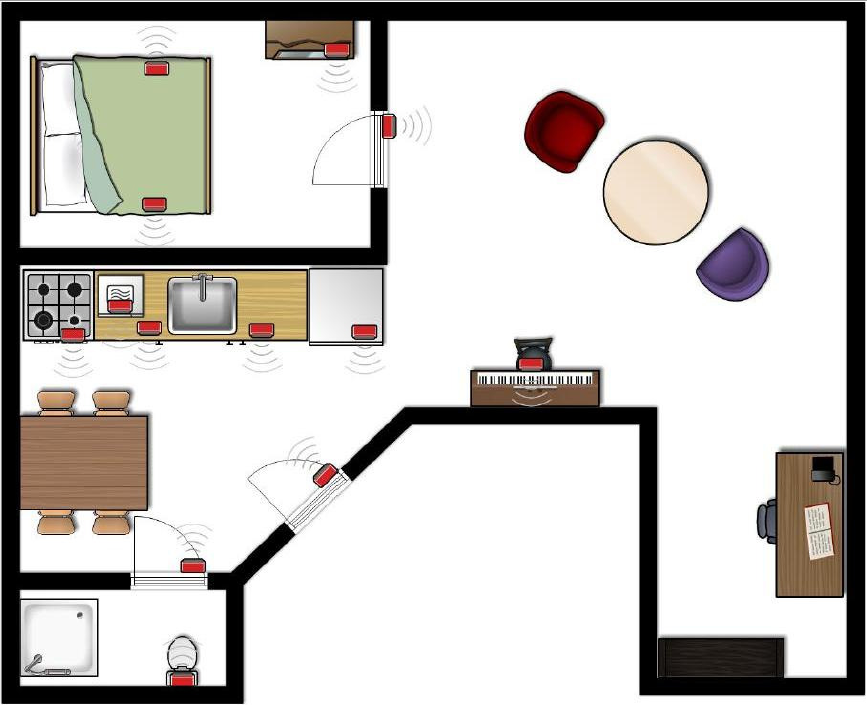
\includegraphics[width=\textwidth]{fig/houseB.png}
		\caption{House B}
		\label{fig:houseB}
	\end{subfigure}
	\\
	\begin{subfigure}[b]{0.35\textwidth}
		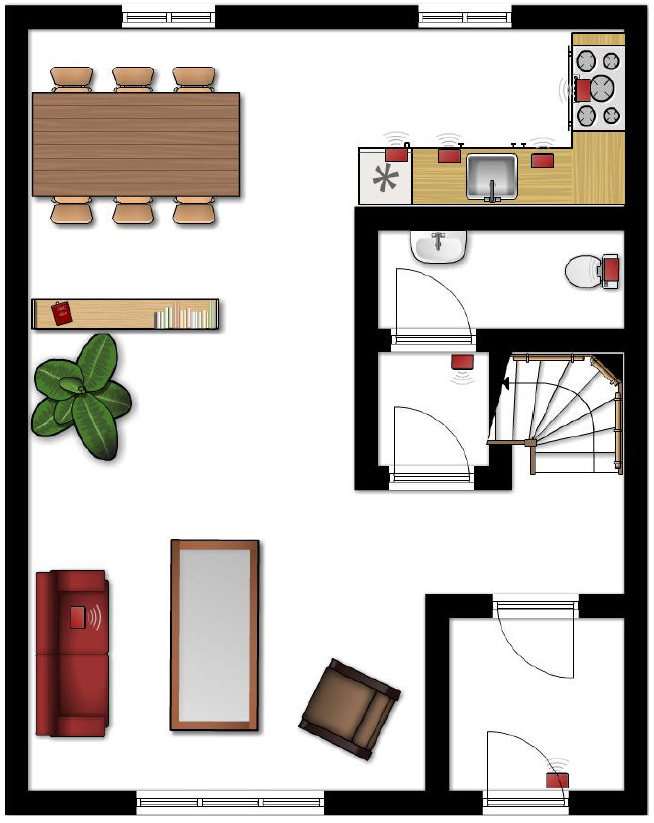
\includegraphics[height=\textwidth,angle=90]{fig/houseC1.png}
		\caption{House C first floor}
		\label{fig:houseC1}
	\end{subfigure}
	~
	\begin{subfigure}[b]{0.35\textwidth}
		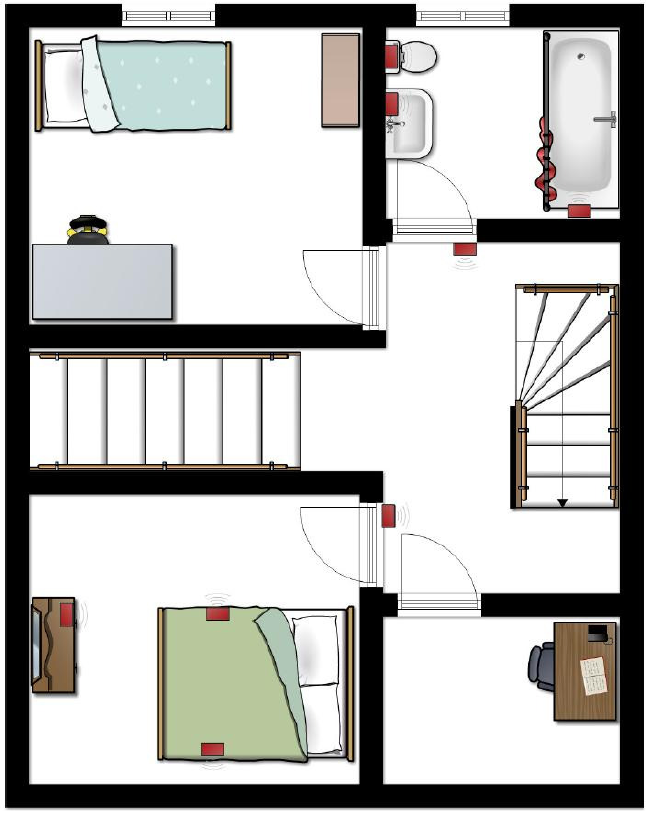
\includegraphics[height=\textwidth,angle=90]{fig/houseC2.png}
		\caption{House C second floor}
		\label{fig:houseC2}
	\end{subfigure}
	\caption{Home floor plans and sensor locations.}\label{fig:houses}
\end{figure}

We evaluate our models on three datasets provided by \cite{tvkasteren2010}.
Figure~\ref{fig:houses} displays the floor plans and sensor locations of the three residences 

The Kasteren dataset is recording a 26-year-old man. He lives alone in a three-room apartment where 14 state-change sensors were installed. Locations of sensors include doors, cup- boards, refrigerator and a toilet flush sensor. Sensors were left unattended, collecting data for 28 days in the apartment. This resulted in 2120 sensor events and 245 activity instances.


%The Kasteren dataset is recording a 26-year-old man. He lives alone in a three-room apartment where 14 state-change sensors were installed. Locations of sensors include doors, cup- boards, refrigerator and a toilet flush sensor. Sensors were left unattended, collecting data for 28 days in the apartment. This resulted in 2120 sensor events and 245 activity instances.
%
%As shown in the table, for Kasteren dataset we have three houses with 14, 23, 21 sensors, respectively.

%The tableis an example of referenced \LaTeX elements.
 
\begin{table*}[t!]
\small
\begin{center}
\begin{tabular}{|c|c|c|c|}
\hline
\textbf{Type} & \emph{House A} & \emph{House B} & \emph{House C}\\ \hline
\textbf{Age} & 26 & 28 & 27\\ \hline
\textbf{Gender} & M & M & M\\ \hline
\textbf{Setting} & Apartment & Apartment & House\\ \hline
\textbf{Room} & 3 & 2 & 6\\ \hline
\textbf{Duration(days)} & 25 & 14 & 19\\ \hline
\textbf{Sensors} & 14 & 23 & 21\\ \hline
\textbf{Activities} & 10 & 13 & 16\\ \hline
\textbf{Annotation} & Bluetooth & Diary & Bluetooh\\ \hline
\end{tabular}
\end{center}
%\vspace{-0.1cm}
\caption{Dataset recording details}
\label{table:datasets}
\vspace{-0.3cm}
\end{table*}




\subsection{Comparative Analysis Metrics}

\begin{equation}
Precision = \frac{TP}{TP+FP}
\end{equation}

\begin{equation}
Recall = \frac{TP}{TP+FN}
\end{equation}

\begin{equation}
Accuracy = \frac{TP+TN}{TP+TN+FP+FN}
\end{equation}

\begin{equation}
F-Measure = \frac{2\cdot Precision\cdot Recall}{Precison+Recall}
\end{equation}

%The Matthews correlation coefficient is used in machine learning as a measure of the quality of binary (two-class) classifications, introduced by biochemist Brian W. Matthews in 1975. It takes into account true and false positives and negatives and is generally regarded as a balanced measure which can be used even if the classes are of very different sizes. The MCC is in essence a correlation coefficient between the observed and predicted binary classifications; it returns a value between ‚àí1 and +1. A coefficient of +1 represents a perfect prediction, 0 no better than random prediction and ‚àí1 indicates total disagreement between prediction and observation.

%\begin{equation}
%MCC=\frac{TP\cdot TN-FP\cdot FN}{\sqrt{(TP+FP)\cdot (TP+FN)\cdot (TN+FP)\cdot (TN+FN)}}
%\end{equation}


\subsection{Discussion}
%\pdfsuppresswarningpagegroup=1
\begin{figure}[t!]
\begin{center}
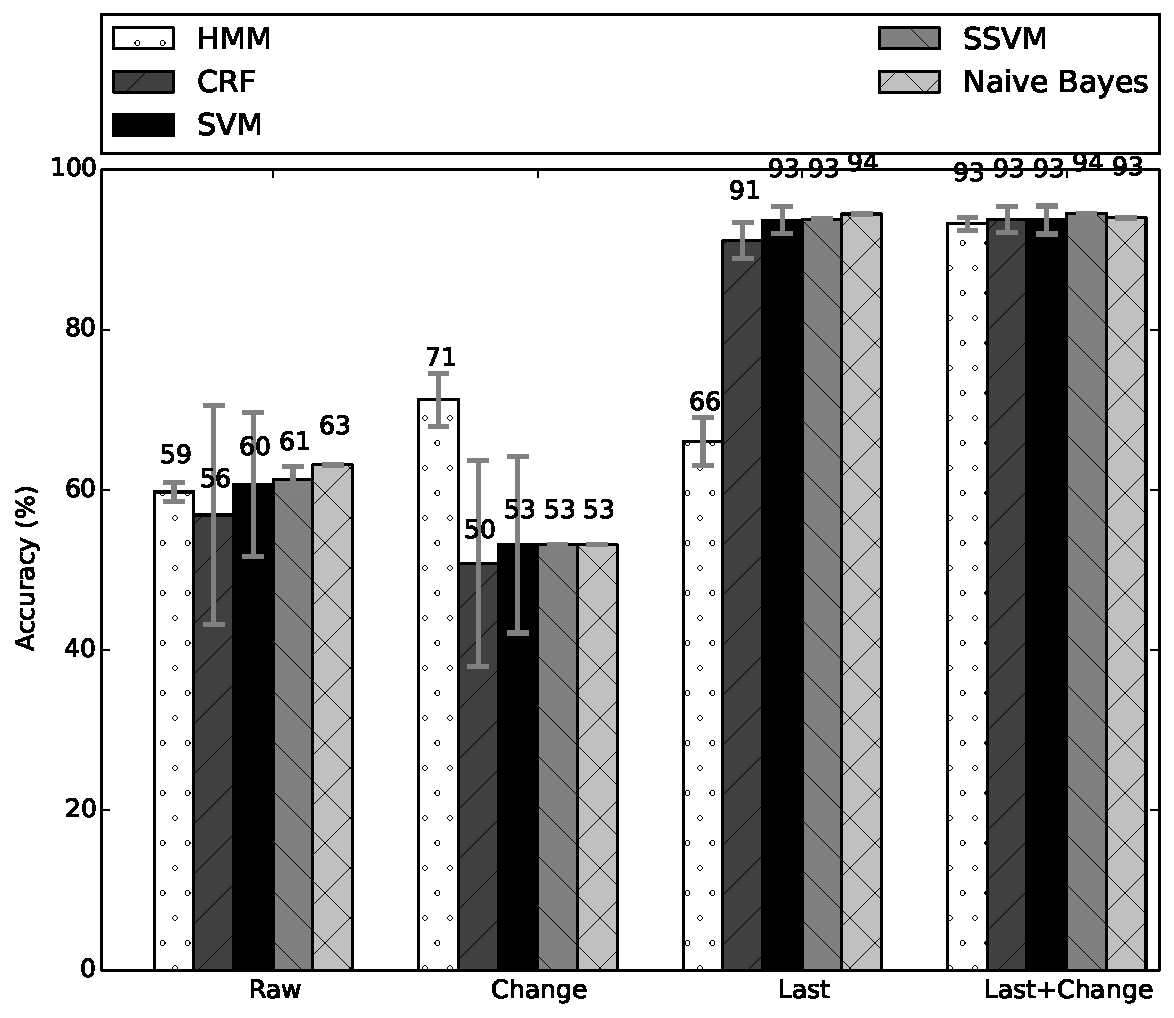
\includegraphics[width=5in]{../../src/reports/A.pdf}
\end{center}
\vspace{-0.5cm}
\caption{House A}
\label{fig:house_a}
\vspace{-0.5cm}
\end{figure}

\begin{figure}[t!]
\begin{center}
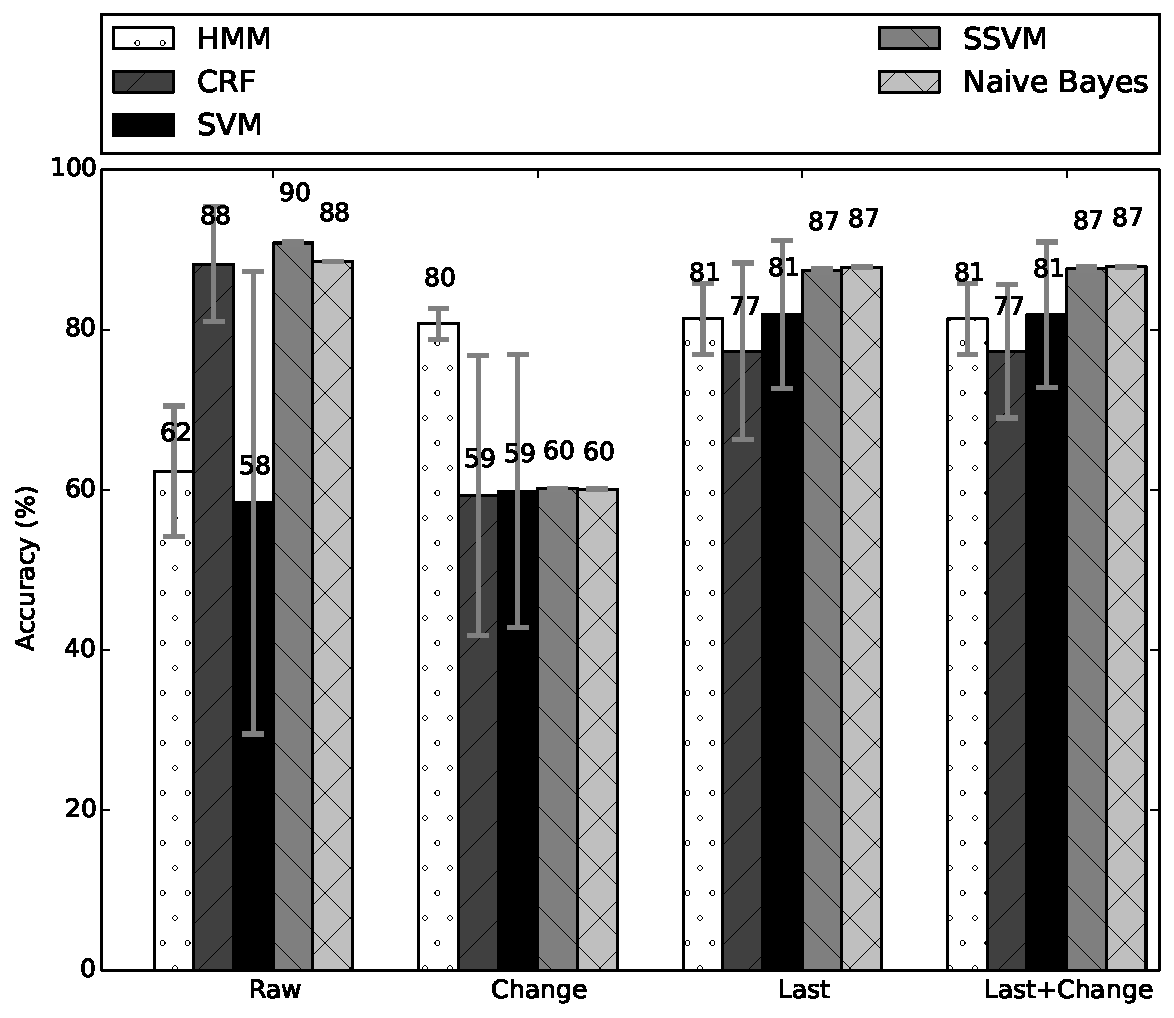
\includegraphics[width=5in]{../../src/reports/B.pdf}
\end{center}
\vspace{-0.5cm}
\caption{House B}
\label{fig:house_b}
\vspace{-0.5cm}
\end{figure}

\begin{figure}[t!]
\begin{center}
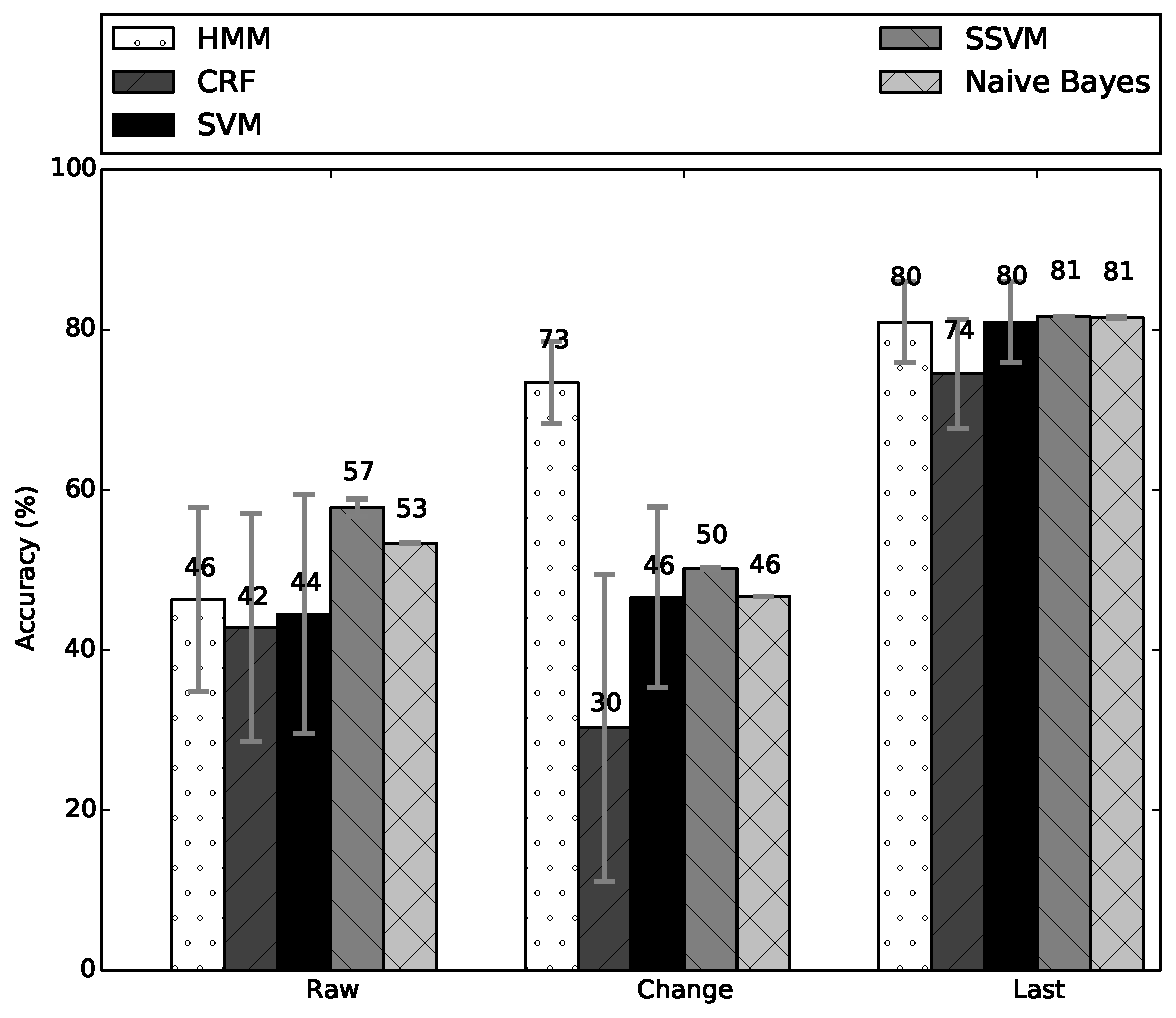
\includegraphics[width=5in]{../../src/reports/C.pdf}
\end{center}
\vspace{-0.5cm}
\caption{House C}
\label{fig:house_3}
\vspace{-0.5cm}
\end{figure}

